\chapter{The (local) Git Pipeline}
\label{chapter:2}

As shortly mentioned in \cref{chapter:1.3.1} the three major parts of your local git project are
\begin{itemize}
	\item the Working Tree or all the files and code you actually write,
	\item the Staging Area or Index where you prepare new content and changes of your work ready to commit and 
	\item the Commit Tree resembling the whole history and development of your project. 
\end{itemize}
These three items make up the stages of the git pipeline which, see xxx versions your whole project in an ongoing process. That is,
you travel through this pipeline again and again. Most of the time the pipe serves for creating new commits. To achieve this, one has to 
travel the pipe from the Working Tree over the Index to the Commit Tree. However, there are occasions where it is helpful to recreate a past state 
of your project (\ac{EG} you want to undo some weird code you have just committed or you want to compare an old status of your work with a new behavior).
No problem, use the git pipeline to load an arbitrary commit from the git Commit Tree and recreate the underlying Working Tree represented.

\begin{figure}[H]
	\centering
	\newcommand*{\xMin}{0}
\newcommand*{\xMax}{14}
\newcommand*{\yMin}{0}
\newcommand*{\yMax}{6}
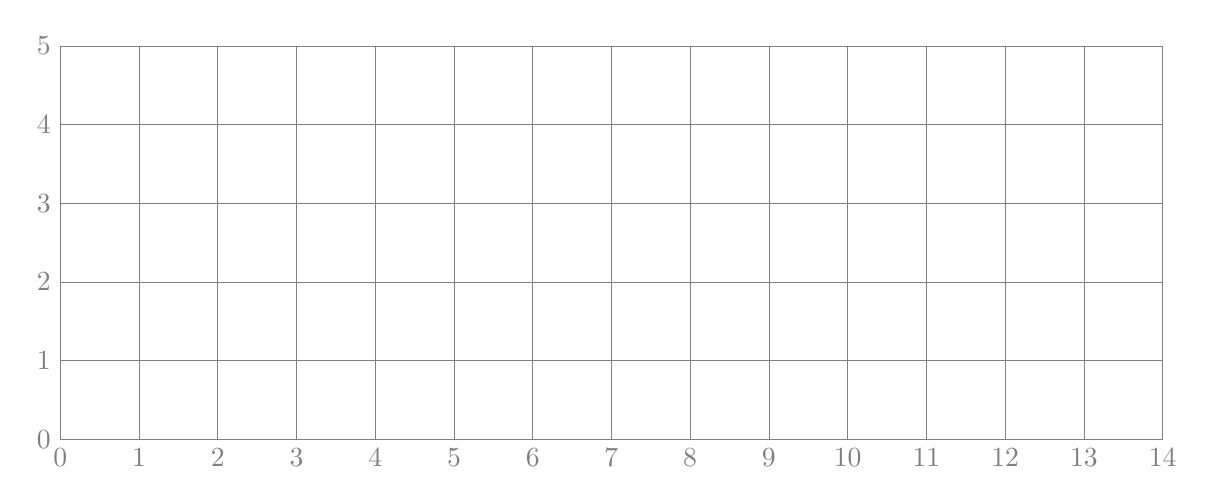
\begin{tikzpicture}
	 \foreach \i in {\xMin,...,\xMax} {
		\draw [very thin,gray] (\i,\yMin) -- (\i,5)  node [below] at (\i,\yMin) {$\i$};
	}
	\foreach \i in {\yMin,...,5
	} {
		\draw [very thin,gray] (\xMin,\i) -- (\xMax,\i) node [left] at (\xMin,\i) {$\i$};
	}
	
	%\draw [step=1.0,blue, very thick] (0.5,0.5) grid (1.5,1.5);
	%\draw [very thick, brown, step=1.0cm,xshift=-0.5cm, yshift=-0.5cm] (0.5,0.5) grid +(1.5,1.5);
	
\end{tikzpicture}
	\caption{The Git Pipeline: Working Tree, Staging Area and Commit Tree}
	\label{fig}
\end{figure}

In other words, the pipeline is the tool or vehicle to append a new commit to the Commit Tree and to reload an already existing one.

 


\section{Commit, HEAD and Branch}
\label{chapter:2.1}


\section{Traveling the Pipeline Forward}
\label{chapter:2.2}


\section{Traveling the Pipeline Backwards}
\label{chapter:2.3}

Hello World!

Finally, an example of how to add literature into the written text \cite{meyers2005effective}.

It is also possible to specify pages with \cite[see][page 127]{arens2015mathematik}.